% ============================================================
\chapter{Gradient Descent and Variants}
\label{ch:gradient}
% ============================================================

\section{Introduction}

In 1847, Augustin-Louis Cauchy proposed an idea of disarming simplicity: to minimize a function, simply follow the direction opposite to the gradient. Like a ball rolling on a surface, one descends the steepest slope, step by step, until reaching the bottom of the valley. This method, \emph{gradient descent}, long remained a theoretical tool. But the explosion of machine learning in the twenty-first century propelled it to the rank of most-executed algorithm in the world: every time a neural network learns, it is a variant of gradient descent that adjusts its billions of parameters. The fundamental questions --- which step size to choose? how to accelerate convergence? what to do when the gradient is too expensive to compute exactly? --- have led to Nesterov's method, Adam, and stochastic gradient descent, which together form the indispensable toolkit of modern optimization.

\section{Fixed Step-Size Gradient Descent}

\begin{algorithme}[title=\textbf{Gradient Descent}]
\begin{enumerate}
    \item Choose $x_0 \in \R^n$, step size $\alpha > 0$.
    \item For $k = 0, 1, 2, \ldots$:
    \[
        x_{k+1} = x_k - \alpha \nabla f(x_k).
    \]
    \item Stop when $\norm{\nabla f(x_k)} < \varepsilon$.
\end{enumerate}
\end{algorithme}

\begin{intuition}
At each iteration, we move in the direction opposite to the gradient (the direction
of steepest local descent) with step size $\alpha$. The gradient points in the
direction of steepest ascent, so $-\nabla f(x_k)$ is the steepest descent direction.
\end{intuition}

\section{Convergence Analysis --- $L$-Smooth Functions}

\begin{theorem}[Convergence for Convex $L$-Smooth Functions]
\label{thm:conv_smooth}
Let $f$ be convex and $L$-smooth. With step size $\alpha = 1/L$:
\[
    f(x_k) - f^* \leq \frac{L\norm{x_0 - x^*}^2}{2k}.
\]
The convergence rate is $O(1/k)$.
\end{theorem}

\begin{proof}
By $L$-smoothness, with $\alpha = 1/L$:
\[
    f(x_{k+1}) \leq f(x_k) + \inner{\nabla f(x_k)}{x_{k+1} - x_k} + \frac{L}{2}\norm{x_{k+1} - x_k}^2.
\]
With $x_{k+1} - x_k = -\frac{1}{L}\nabla f(x_k)$:
\[
    f(x_{k+1}) \leq f(x_k) - \frac{1}{2L}\norm{\nabla f(x_k)}^2.
\]

By the first-order condition: $f(x_k) - f^* \leq \inner{\nabla f(x_k)}{x_k - x^*}
\leq \norm{\nabla f(x_k)}\norm{x_k - x^*}$, so:
\[
    \norm{\nabla f(x_k)}^2 \geq \frac{(f(x_k) - f^*)^2}{\norm{x_k - x^*}^2}.
\]

Moreover, $\norm{x_{k+1} - x^*}^2 = \norm{x_k - x^*}^2 - \frac{2}{L}\inner{\nabla f(x_k)}{x_k - x^*} + \frac{1}{L^2}\norm{\nabla f(x_k)}^2$.

Setting $\delta_k = f(x_k) - f^*$ and $R_k = \norm{x_k - x^*}^2$:
\[
    \delta_{k+1} \leq \delta_k - \frac{1}{2L}\norm{\nabla f(x_k)}^2, \quad
    R_{k+1} \leq R_k - \frac{2}{L}\delta_k + \frac{1}{L^2}\norm{\nabla f(x_k)}^2.
\]

Summing the sufficient decrease:
$\sum_{i=0}^{k-1} \frac{1}{2L}\norm{\nabla f(x_i)}^2 \leq \delta_0$, and by a
telescoping argument on $R_k$:
\[
    \sum_{i=0}^{k-1} \delta_i \leq \frac{L}{2}R_0.
\]
Since $\delta_k$ is decreasing: $k\delta_k \leq \sum_{i=0}^{k-1}\delta_i \leq \frac{L}{2}R_0$.
\end{proof}

\section{Convergence for Strongly Convex Functions}

\begin{theorem}[Linear Convergence]
\label{thm:conv_strong}
Let $f$ be $m$-strongly convex and $L$-smooth. With $\alpha = 1/L$:
\[
    f(x_k) - f^* \leq \left(1 - \frac{m}{L}\right)^k (f(x_0) - f^*).
\]
The rate is linear (geometric convergence) with factor $1 - 1/\kappa$ where
$\kappa = L/m$ is the condition number.
\end{theorem}

\begin{proof}
By $L$-smoothness and step $\alpha = 1/L$:
$f(x_{k+1}) \leq f(x_k) - \frac{1}{2L}\norm{\nabla f(x_k)}^2$.

By strong convexity: $\norm{\nabla f(x_k)}^2 \geq 2m(f(x_k) - f^*)$
(Polyak--\L{}ojasiewicz inequality). Thus:
\[
    f(x_{k+1}) - f^* \leq (f(x_k) - f^*) - \frac{m}{L}(f(x_k) - f^*)
    = \left(1 - \frac{m}{L}\right)(f(x_k) - f^*).
\]
\end{proof}

\begin{keyformulas}[title=\textbf{Convergence Rate Summary}]
\begin{center}
\renewcommand{\arraystretch}{1.3}
\begin{tabular}{lcc}
\toprule
\textbf{Assumption} & \textbf{Rate} & \textbf{Complexity for $\varepsilon$} \\
\midrule
Convex, $L$-smooth & $O(1/k)$ & $O(L/\varepsilon)$ \\
$m$-str.\ convex, $L$-smooth & $O((1-m/L)^k)$ & $O(\kappa\log(1/\varepsilon))$ \\
Convex, nonsmooth & $O(1/\sqrt{k})$ & $O(1/\varepsilon^2)$ \\
\bottomrule
\end{tabular}
\end{center}
\end{keyformulas}

\section{Line Search}

\begin{definition}[Armijo Condition (Backtracking)]
Choose $\alpha_k$ as the largest $\alpha = \beta^j \hat{\alpha}$ ($j = 0,1,\ldots$)
satisfying:
\[
    f(x_k - \alpha\nabla f(x_k)) \leq f(x_k) - c\alpha\norm{\nabla f(x_k)}^2,
\]
with $c \in (0, 1/2)$ and $\beta \in (0,1)$.
\end{definition}

\begin{proposition}
Gradient descent with Armijo backtracking preserves the same convergence rates
$O(1/k)$ and $O((1-m/L)^k)$ (with different constants).
\end{proposition}

\section{Nesterov's Accelerated Gradient}

\begin{algorithme}[title=\textbf{Nesterov's Accelerated Gradient (NAG)}]
\begin{enumerate}
    \item Initialize $x_0 = y_0 \in \R^n$.
    \item For $k = 0, 1, 2, \ldots$:
    \begin{align*}
        x_{k+1} &= y_k - \frac{1}{L}\nabla f(y_k), \\
        y_{k+1} &= x_{k+1} + \frac{k}{k+3}(x_{k+1} - x_k).
    \end{align*}
\end{enumerate}
\end{algorithme}

\begin{theorem}[Nesterov's Convergence]
\label{thm:nesterov}
Let $f$ be convex and $L$-smooth. Nesterov's algorithm satisfies:
\[
    f(x_k) - f^* \leq \frac{2L\norm{x_0 - x^*}^2}{(k+1)^2}.
\]
The rate $O(1/k^2)$ is optimal among first-order methods
(Nemirovski--Yudin lower bound).
\end{theorem}

\begin{warning}[title=\textbf{Optimality of the $O(1/k^2)$ Rate}]
Nemirovski and Yudin (1983) showed that no first-order method (using only values of
$f$ and $\nabla f$) can converge faster than $O(1/k^2)$ for the class of convex
$L$-smooth functions. Nesterov's acceleration achieves this bound: it is \emph{optimal}.
\end{warning}

\section{Conjugate Gradient}

\begin{algorithme}[title=\textbf{Nonlinear Conjugate Gradient (Fletcher--Reeves)}]
\begin{enumerate}
    \item $d_0 = -\nabla f(x_0)$.
    \item For $k = 0, 1, 2, \ldots$:
    \begin{enumerate}
        \item $\alpha_k = \argmin_{\alpha > 0} f(x_k + \alpha d_k)$.
        \item $x_{k+1} = x_k + \alpha_k d_k$.
        \item $\beta_{k+1} = \frac{\norm{\nabla f(x_{k+1})}^2}{\norm{\nabla f(x_k)}^2}$.
        \item $d_{k+1} = -\nabla f(x_{k+1}) + \beta_{k+1} d_k$.
    \end{enumerate}
\end{enumerate}
\end{algorithme}

\begin{remark}
For a quadratic function $f(x) = \frac{1}{2}x^TAx - b^Tx$ with $A \succ 0$,
conjugate gradient converges in at most $n$ iterations (finite convergence).
\end{remark}

\section{Stochastic Gradient Descent (SGD)}

\begin{algorithme}[title=\textbf{Stochastic Gradient Descent}]
For $f(x) = \frac{1}{N}\sum_{i=1}^N f_i(x)$:
\begin{enumerate}
    \item For $k = 0, 1, 2, \ldots$:
    \begin{enumerate}
        \item Sample $i_k$ uniformly from $\{1, \ldots, N\}$.
        \item $x_{k+1} = x_k - \alpha_k \nabla f_{i_k}(x_k)$.
    \end{enumerate}
\end{enumerate}
\end{algorithme}

\begin{theorem}[SGD Convergence]
For convex, $L$-smooth $f$, with
$\mathbb{E}[\norm{\nabla f_i(x) - \nabla f(x)}^2] \leq \sigma^2$ and
$\alpha_k = c/\sqrt{k}$:
\[
    \mathbb{E}[f(\bar{x}_k)] - f^* = O\left(\frac{1}{\sqrt{k}}\right),
\]
where $\bar{x}_k = \frac{1}{k}\sum_{i=1}^k x_i$. For $m$-strongly convex $f$ with
$\alpha_k = 1/(mk)$:
\[
    \mathbb{E}[f(\bar{x}_k)] - f^* = O\left(\frac{1}{k}\right).
\]
\end{theorem}

\section{Modern SGD Variants}

\begin{algorithme}[title=\textbf{Adam (Kingma \& Ba, 2015)}]
\begin{enumerate}
    \item Parameters: $\beta_1 = 0.9$, $\beta_2 = 0.999$, $\varepsilon = 10^{-8}$, $\alpha$.
    \item $m_0 = 0$, $v_0 = 0$.
    \item For $k = 1, 2, \ldots$:
    \begin{align*}
        g_k &= \nabla f_{i_k}(x_k), \\
        m_k &= \beta_1 m_{k-1} + (1-\beta_1) g_k, \\
        v_k &= \beta_2 v_{k-1} + (1-\beta_2) g_k^2, \\
        \hat{m}_k &= m_k / (1 - \beta_1^k), \\
        \hat{v}_k &= v_k / (1 - \beta_2^k), \\
        x_{k+1} &= x_k - \alpha \hat{m}_k / (\sqrt{\hat{v}_k} + \varepsilon).
    \end{align*}
\end{enumerate}
\end{algorithme}

\section{Geometric Interpretation}

\begin{center}
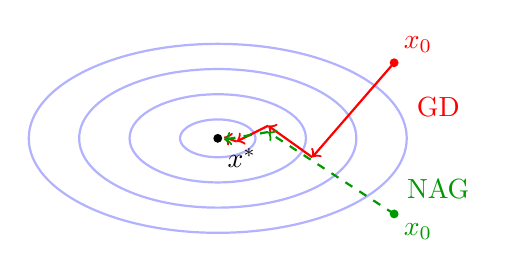
\begin{tikzpicture}[scale=0.8]
    % Contour lines of quadratic
    \draw[blue!30, thick] (0,0) ellipse (3 and 1.5);
    \draw[blue!30, thick] (0,0) ellipse (2.2 and 1.1);
    \draw[blue!30, thick] (0,0) ellipse (1.4 and 0.7);
    \draw[blue!30, thick] (0,0) ellipse (0.6 and 0.3);

    % Gradient descent path
    \draw[->, thick, red] (2.8, 1.2) -- (1.5, -0.3);
    \draw[->, thick, red] (1.5, -0.3) -- (0.8, 0.2);
    \draw[->, thick, red] (0.8, 0.2) -- (0.3, -0.05);
    \draw[->, thick, red] (0.3, -0.05) -- (0.1, 0.02);

    \fill[red] (2.8, 1.2) circle (2pt) node[above right] {$x_0$};
    \fill[black] (0,0) circle (2pt) node[below right] {$x^*$};

    % Nesterov path
    \draw[->, thick, green!60!black, dashed] (2.8, -1.2) -- (0.8, 0.1);
    \draw[->, thick, green!60!black, dashed] (0.8, 0.1) -- (0.1, -0.02);

    \fill[green!60!black] (2.8, -1.2) circle (2pt) node[below right] {$x_0$};

    \node[red] at (3.5, 0.5) {GD};
    \node[green!60!black] at (3.5, -0.8) {NAG};
\end{tikzpicture}
\end{center}

\section{Python Implementation}

\begin{codeblock}[title=\textbf{Comparison of GD, Nesterov, and SGD}]
\begin{minted}{python}
import numpy as np
import matplotlib.pyplot as plt

def gradient_descent(f, grad_f, x0, L, n_iter):
    x = x0.copy()
    history = [f(x)]
    for k in range(n_iter):
        x = x - (1/L) * grad_f(x)
        history.append(f(x))
    return x, history

def nesterov_accelerated(f, grad_f, x0, L, n_iter):
    x = x0.copy()
    y = x0.copy()
    history = [f(x)]
    for k in range(n_iter):
        x_new = y - (1/L) * grad_f(y)
        y = x_new + (k / (k + 3)) * (x_new - x)
        x = x_new
        history.append(f(x))
    return x, history

# Ill-conditioned quadratic
np.random.seed(42)
n = 50
eigvals = np.logspace(-2, 2, n)  # kappa = 10000
Q_diag = eigvals
b = np.random.randn(n)

f = lambda x: 0.5 * np.sum(Q_diag * x**2) - np.sum(b * x)
grad_f = lambda x: Q_diag * x - b
L = np.max(Q_diag)
f_star = -0.5 * np.sum(b**2 / Q_diag)

x0 = np.zeros(n)
_, hist_gd = gradient_descent(f, grad_f, x0, L, 500)
_, hist_nag = nesterov_accelerated(f, grad_f, x0, L, 500)

plt.semilogy(np.array(hist_gd) - f_star, label='GD')
plt.semilogy(np.array(hist_nag) - f_star, label='Nesterov')
plt.xlabel('Iteration k')
plt.ylabel('$f(x_k) - f^*$')
plt.legend()
plt.title('GD vs Nesterov (kappa=10000)')
plt.grid(True, alpha=0.3)
plt.savefig('gd_vs_nesterov.pdf')
\end{minted}
\end{codeblock}

\section{Exercises}

\begin{exercise}[$\star$]
Show that for $f(x) = \frac{1}{2}\norm{Ax-b}^2$, the gradient is
$\nabla f(x) = A^T(Ax-b)$ and the smoothness constant is $L = \norm{A^TA}$.
\end{exercise}

\begin{exercise}[$\star\star$]
Prove the Polyak--\L{}ojasiewicz inequality: if $f$ is $m$-strongly convex, then
$\norm{\nabla f(x)}^2 \geq 2m(f(x) - f^*)$.
\end{exercise}

\begin{exercise}[$\star\star$]
Implement Armijo backtracking and compare with fixed step $1/L$ on a logistic
regression problem.
\end{exercise}

\begin{exercise}[$\star\star$]
Show that conjugate gradient converges in at most $n$ iterations for a quadratic in
dimension $n$.
\end{exercise}

\begin{exercise}[$\star\star\star$]
Prove the $O(1/k^2)$ convergence bound of Nesterov's accelerated gradient using a
Lyapunov function.
\end{exercise}

\begin{exercise}[$\star\star\star$]
Show the Nemirovski--Yudin lower bound: there exists a convex $L$-smooth function
such that any first-order method satisfies
$f(x_k) - f^* \geq \frac{cL\norm{x_0-x^*}^2}{k^2}$ for $k \leq (n-1)/2$.
\end{exercise}
